\documentclass[conference]{IEEEtran}
\usepackage{cite}
\usepackage{amsmath,amssymb,amsfonts}
\usepackage{algorithmic}
\usepackage{graphicx}
\usepackage{textcomp}
\usepackage{xcolor}
\usepackage{booktabs}
\usepackage{url}
\usepackage{hyperref}

\hypersetup{
    colorlinks=true,
    linkcolor=blue,
    citecolor=blue,
    urlcolor=blue
}

\begin{document}

\title{Fixed-$k$ versus Score-Gap Adaptive-$k$ Proxy Context Selection for Multi-Hop QA:\\An Evidence-Coverage and Token-Efficiency Study}

\author{\IEEEauthorblockN{Pranav Kumar Gupta}
\IEEEauthorblockA{\textit{Department of Information Technology} \\
\textit{Indian Institute of Information Technology Allahabad}\\
Prayagraj, India \\
MHM2026012@iiita.ac.in}
}

\maketitle

\begin{abstract}
Retrieval-Augmented Generation (RAG) systems select relevant passages from external knowledge sources to reduce the amount of context supplied to downstream language models. However, standard RAG pipelines often rely on static passage budgets (fixed-$k$), creating a trade-off between retrieving sufficient supporting evidence for multi-hop questions and selecting additional non-gold paragraphs that increase context size. Recently, single-pass Adaptive-$k$ selection based on discrete score drops has been proposed to optimize retrieval budgets without model fine-tuning. In this work, we conduct a controlled comparative study (Pathway B) investigating fixed-$k$ ($k \in \{1, 3, 5, 10\}$) versus Score-Gap Adaptive-$k$ Proxy context selection on the multi-hop HotpotQA benchmark across two sparse retrieval paradigms: BM25 and TF-IDF. Evaluating 500 verified questions under pre-frozen decision rules with 95\% bootstrap confidence intervals, we find that Adaptive-$k$ dynamically selects $k \approx 2.02$--$2.22$ paragraphs, achieving substantial token reductions (78.5\% fewer tokens than full context and 26.1\% fewer than fixed $k=3$) while maintaining high precision (73.9\% for BM25; 77.0\% for TF-IDF). However, contrary to the hypothesis that Adaptive-$k$ matches fixed $k=5$ multi-hop coverage, Adaptive-$k$ achieves only 21.4\% full coverage on multi-evidence questions compared to 61.6\% for fixed $k=5$. Qualitative analysis of 40 sampled missed-evidence cases shows that 55\% ($N=22$) were categorized as cases where bridge entities were absent from the query text. This failure pattern was associated with early score drops and the exclusion of second-hop evidence paragraphs. These findings indicate that Adaptive-$k$ achieves higher full coverage on comparison questions (29.3\%) than on bridge questions (19.6\%) under BM25, although its overall multi-evidence coverage remains below fixed $k=5$. The results suggest that iterative query reformulation is a direction worth investigating for improving retrieval of second-hop evidence.
\end{abstract}

\begin{IEEEkeywords}
Information Retrieval, Multi-Hop Question Answering, Retrieval-Augmented Generation, Adaptive Context Selection, Token Efficiency, Evidence Coverage.
\end{IEEEkeywords}

\section{Introduction}
Large language models (LLMs) have achieved unprecedented context window capacities, theoretically allowing prompt lengths exceeding tens of thousands of tokens. However, empirical studies demonstrate that nominal sequence capacity does not guarantee effective information utilization. Under the well-documented ``Lost in the Middle'' phenomenon, models suffer severe degradation in retrieval fidelity and reasoning accuracy when key factual evidence is situated in the interior of extensive contexts~\cite{liu2024lost}. Furthermore, recent evaluations such as NoLiMa~\cite{modarressi2025nolima} and Maximum Effective Context Window (MECW) analyses~\cite{paulsen2026context} confirm that when lexical shortcuts are eliminated, practical reasoning degrades at sequence lengths far shorter than advertised maximums.

Retrieval-Augmented Generation (RAG) provides a natural architectural mitigation by selectively retrieving relevant passages from an external corpus and presenting only top-ranked chunks to the reader~\cite{lewis2020rag, zhao2024longrag}. Yet, traditional RAG pipelines rely on a static number of retrieved passages (fixed-$k$). This design introduces a fundamental dilemma:
\begin{enumerate}
    \item \textbf{Under-retrieval ($k$ too small)}: Selecting too few paragraphs can exclude necessary supporting evidence from multi-hop questions, reducing the full evidence coverage achieved by the retrieval system.
    \item \textbf{Over-retrieval ($k$ too large)}: Selecting additional non-gold paragraphs increases the number of retrieved tokens and can reduce paragraph-level precision. The effects of additional context on downstream model latency and positional retrieval degradation are outside the scope of this study.
\end{enumerate}

To address this challenge, Taguchi et al.~\cite{taguchi2025adaptivek} introduced \textit{Adaptive-$k$}, a single-pass context selection method that determines query-specific passage cutoffs based on the largest discrete drop in similarity score distributions. Prior work reports that Adaptive-$k$ can match fixed-$k$ reader accuracy with up to $10\times$ fewer tokens on dense retrievers. However, the behavior of single-pass score-drop selection on sparse retrieval backends and its paragraph-level evidence coverage on multi-evidence questions remain to be investigated.

In this paper, we conduct a controlled comparative evaluation (Pathway B) comparing fixed-$k$ ($k \in \{1, 3, 5, 10\}$) against Score-Gap Adaptive-$k$ Proxy across BM25 and TF-IDF retrievers on the HotpotQA distractor validation split ($N=500$)~\cite{yang2018hotpotqa}. The evaluation focuses exclusively on retrieval-level evidence coverage, paragraph-level precision, token consumption, and retrieval and selection latency. Adhering to strict reproducibility directives, all protocols and decision rules were frozen prior to viewing experimental results, and all metrics are reported with 95\% bootstrap confidence intervals.

\section{Related Work}
\subsection{Context-Window Degradation and Positional Bias}
Transformer attention scales quadratically with sequence length, but empirical failures are primarily driven by learned positional attention bias and distractor interference~\cite{liu2024lost, hsieh2024found}. Liu et al.~\cite{liu2024lost} showed that language model performance follows a U-shaped curve: accuracy is highest when relevant information is at the extreme beginning or end of the input context, falling precipitously when evidence is located mid-context. 

Paulsen~\cite{paulsen2026context} formalized the Maximum Effective Context Window (MECW), proving that effective reasoning capacity can degrade by up to 99\% of nominal context limits, with severe degradation initiating around $\sim 1,000$ tokens for multi-step reasoning. Similarly, Modarressi et al.~\cite{modarressi2025nolima} demonstrated that in the absence of exact keyword overlap, 11 out of 13 evaluated frontier models drop below 50\% retrieval success at 32K tokens. DENIAHL~\cite{dai2024deniahl} further demonstrated that in-context feature placement and distractor density dictate needle recovery.

These studies provide background on context-window degradation and positional bias; neither phenomenon is directly evaluated in the present retrieval-only experiments.

\subsection{Context Selection in RAG Pipelines}
To shield LLMs from distractor saturation, RAG restricts prompt size to relevant passages~\cite{lewis2020rag}. However, traditional fixed-$k$ heuristics fail to accommodate query variance. Iterative routing approaches such as Self-RAG or iterative decomposition may require multiple model inference calls. Their effects on downstream inference latency are not evaluated in the present study. 

LongRAG~\cite{zhao2024longrag} proposed scaling retrieval units to 4K tokens to balance global context with local details, yielding up to 17.25\% gains on multi-hop benchmarks. Conversely, Taguchi et al.~\cite{taguchi2025adaptivek} introduced Adaptive-$k$, demonstrating that evaluating the first discrete differences between sorted passage similarity scores allows single-pass dynamic truncation without model fine-tuning.

\section{Methodology}
\subsection{Task Formulation}
Let $q$ denote an input question, and let $\mathcal{P} = \{p_1, p_2, \dots, p_M\}$ be a candidate pool of $M=10$ candidate paragraphs containing a subset of gold supporting paragraphs $\mathcal{P}_{\text{gold}} \subset \mathcal{P}$ ($|\mathcal{P}_{\text{gold}}| \ge 2$ in HotpotQA). A retriever $R$ computes similarity scores $s(q, p_i)$ for all $p_i \in \mathcal{P}$, producing a permutation of indices sorted in descending order of relevance:
\begin{equation}
    \pi = (\pi_1, \pi_2, \dots, \pi_M), \quad s(q, p_{\pi_1}) \ge s(q, p_{\pi_2}) \ge \dots \ge s(q, p_{\pi_M})
\end{equation}

\subsection{Retrievers}
We evaluate two classical sparse retrieval paradigms:
\begin{enumerate}
    \item \textbf{BM25 (Okapi)}: Probabilistic term matching weighted by inverse document frequency and paragraph length normalization:
    \begin{equation}
        \text{BM25}(q, p) = \sum_{w \in q} \text{IDF}(w) \cdot \frac{f(w, p) \cdot (k_1 + 1)}{f(w, p) + k_1 \cdot (1 - b + b \cdot \frac{|p|}{\text{avgdl}})}
    \end{equation}
    with standard parameters $k_1 = 1.5, b = 0.75$.
    \item \textbf{TF-IDF Cosine}: Vector-space representation with sublinear term-frequency scaling ($1 + \log(\text{tf})$) and cosine similarity between query and document vectors.
\end{enumerate}

\subsection{Context Selection Strategies}
\begin{enumerate}
    \item \textbf{Fixed-$k$}: Selects the prefix of top-$k$ ranked paragraphs: $\mathcal{S}_{\text{fixed}}(k) = \{\pi_1, \dots, \pi_k\}$ for $k \in \{1, 3, 5, 10\}$.
    \item \textbf{Score-Gap Adaptive-$k$ Proxy}: Following Taguchi et al.~\cite{taguchi2025adaptivek}, the cutoff $k^*$ is determined by finding the maximum discrete gap between consecutive sorted scores:
    \begin{equation}
        k^* = \arg\max_{i \in \{1, \dots, M-1\}} \left( s(q, p_{\pi_i}) - s(q, p_{\pi_{i+1}}) \right)
    \end{equation}
    If scores are degenerate or uniform ($\max_i \Delta s_i \le 0$), a fallback $k^* = 3$ is assigned. The selected context is $\mathcal{S}_{\text{adapt}} = \{\pi_1, \dots, \pi_{k^*}\}$.
\end{enumerate}

\section{Experimental Setup}
\subsection{Dataset and Preprocessing}
We utilize the validation set of HotpotQA in the distractor setting~\cite{yang2018hotpotqa}. In this setting, each question is paired with exactly 10 candidate Wikipedia paragraphs (2 gold supporting paragraphs and 8 hard distractors selected via TF-IDF). We inspect and validate the first 500 valid samples deterministically. During data ingestion, five corrupted records containing fewer than 10 candidate paragraphs were identified and skipped, yielding exactly 500 validated questions (408 bridge questions, 92 comparison questions).

\subsection{Leakage Prevention}
To prevent gold-label information from influencing retrieval, candidate paragraphs were stripped of all `is\_gold` annotations and title metadata before scoring. Unit tests showed that retrieval rankings remained unchanged when gold fields were blanked.

\subsection{Evaluation Metrics}
\begin{itemize}
    \item \textbf{Evidence Recall} ($\uparrow$): Fraction of gold paragraphs retrieved: $\frac{|\mathcal{S} \cap \mathcal{P}_{\text{gold}}|}{|\mathcal{P}_{\text{gold}}|}$.
    \item \textbf{Full-Coverage Rate} ($\uparrow$): Binary indicator whether 100\% of gold paragraphs were selected: $\mathbb{I}(\mathcal{P}_{\text{gold}} \subseteq \mathcal{S})$.
    \item \textbf{Precision} ($\uparrow$): Fraction of selected paragraphs that are gold: $\frac{|\mathcal{S} \cap \mathcal{P}_{\text{gold}}|}{|\mathcal{S}|}$.
    \item \textbf{Estimated Tokens} ($\downarrow$): Estimated token count obtained by multiplying whitespace word counts by $1.3$.
    \item \textbf{Coverage per 1k Tokens} ($\uparrow$): Primary token efficiency metric: $\frac{\text{Evidence Recall}}{\text{Selected Tokens}} \times 1000$.
    \item \textbf{Selection Latency} ($\downarrow$): Wall-clock retrieval and selection latency in milliseconds.
\end{itemize}
All metrics are reported as mean values with 95\% percentile bootstrap confidence intervals computed over 1,000 resamples (seed 0).

\section{Results}

\begin{table*}[t]
\centering
\caption{Main Evaluation Results on HotpotQA Validation (500 Questions). Mean values with 95\% Bootstrap Confidence Intervals (1,000 resamples).}
\label{tab:main_results}
\begin{tabular}{llrcccccc}
\toprule
\textbf{Retriever} & \textbf{Method} & \textbf{Mean $k$} & \textbf{Evidence Recall} & \textbf{Full Coverage \%} & \textbf{Precision} & \textbf{Estimated Tokens} & \textbf{Latency (ms)} & \textbf{Cov / 1k Tokens} \\
\midrule
BM25 & Fixed $k=1$ & 1.00 & 0.404 [0.386, 0.421] & \phantom{0}0.0\% [\phantom{0}0.0\%, \phantom{0}0.0\%] & 0.808 [0.772, 0.842] & 101.8 [96.4, 108.0] & 0.64 [0.62, 0.65] & 5.714 [5.333, 6.090] \\
BM25 & Fixed $k=3$ & 3.00 & 0.709 [0.683, 0.733] & 45.6\% [40.8\%, 50.0\%] & 0.473 [0.455, 0.489] & 356.2 [343.6, 371.3] & 0.63 [0.62, 0.65] & 2.310 [2.194, 2.431] \\
BM25 & Fixed $k=5$ & 5.00 & 0.801 [0.780, 0.822] & 61.6\% [57.4\%, 65.6\%] & 0.320 [0.312, 0.329] & 616.0 [598.0, 634.6] & 0.63 [0.62, 0.65] & 1.442 [1.385, 1.503] \\
BM25 & Fixed $k=10$ & 10.00 & 1.000 [1.000, 1.000] & 100.0\% [100.0\%, 100.0\%] & 0.200 [0.200, 0.200] & 1226.8 [1198.8, 1256.6] & 0.63 [0.62, 0.65] & 0.870 [0.849, 0.892] \\
BM25 & Score-Gap Adaptive-$k$ Proxy & 2.22 & 0.568 [0.545, 0.591] & 21.4\% [17.8\%, 25.2\%] & 0.739 [0.706, 0.769] & 263.2 [235.4, 293.8] & 0.68 [0.66, 0.69] & 4.925 [4.561, 5.295] \\
\midrule
TF-IDF & Fixed $k=1$ & 1.00 & 0.413 [0.396, 0.429] & \phantom{0}0.0\% [\phantom{0}0.0\%, \phantom{0}0.0\%] & 0.826 [0.792, 0.858] & \phantom{0}84.9 [81.0, 89.0] & 1.89 [1.85, 1.93] & 6.388 [5.973, 6.807] \\
TF-IDF & Fixed $k=3$ & 3.00 & 0.723 [0.697, 0.748] & 49.8\% [45.4\%, 54.0\%] & 0.482 [0.465, 0.499] & 297.9 [289.0, 306.9] & 1.89 [1.85, 1.93] & 2.791 [2.645, 2.942] \\
TF-IDF & Fixed $k=5$ & 5.00 & 0.831 [0.810, 0.853] & 67.2\% [63.2\%, 71.4\%] & 0.332 [0.324, 0.341] & 538.7 [526.1, 551.8] & 1.89 [1.85, 1.93] & 1.679 [1.613, 1.744] \\
TF-IDF & Fixed $k=10$ & 10.00 & 1.000 [1.000, 1.000] & 100.0\% [100.0\%, 100.0\%] & 0.200 [0.200, 0.200] & 1226.8 [1198.8, 1256.6] & 1.89 [1.85, 1.93] & 0.870 [0.849, 0.892] \\
TF-IDF & Score-Gap Adaptive-$k$ Proxy & 2.02 & 0.574 [0.550, 0.596] & 23.2\% [19.6\%, 26.8\%] & 0.770 [0.737, 0.799] & 200.6 [179.2, 227.1] & 1.94 [1.90, 1.98] & 5.820 [5.426, 6.229] \\
\bottomrule
\end{tabular}
\end{table*}

\subsection{Main Findings (Table~\ref{tab:main_results})}
Table~\ref{tab:main_results} reports performance across all 10 experimental conditions. 
\begin{enumerate}
    \item \textbf{Context Token Reduction}: Score-Gap Adaptive-$k$ Proxy dynamically selects an average of $k=2.22$ paragraphs for BM25 (263.2 tokens) and $k=2.02$ paragraphs for TF-IDF (200.6 tokens). This achieves a 78.5\% token reduction relative to full context ($k=10$, 1226.8 tokens) and a 26.1\% reduction relative to fixed $k=3$ (356.2 tokens).
    \item \textbf{Precision and Distractor Suppression}: Score-Gap Adaptive-$k$ Proxy maintains high precision: 0.739 for BM25 and 0.770 for TF-IDF. By comparison, fixed $k=5$ achieves 0.320 paragraph-level precision. In the 10-paragraph HotpotQA distractor setting, this indicates that approximately two-thirds of the five selected paragraphs are non-gold distractors; this is a paragraph-level observation rather than a token-level estimate.
    \item \textbf{Efficiency Frontier}: In terms of coverage per 1,000 tokens, Score-Gap Adaptive-$k$ Proxy yields 4.925 for BM25 and 5.820 for TF-IDF, significantly surpassing fixed $k=3$ (2.310 and 2.791) and fixed $k=5$ (1.442 and 1.679).
\end{enumerate}

\begin{figure}[t]
\centering
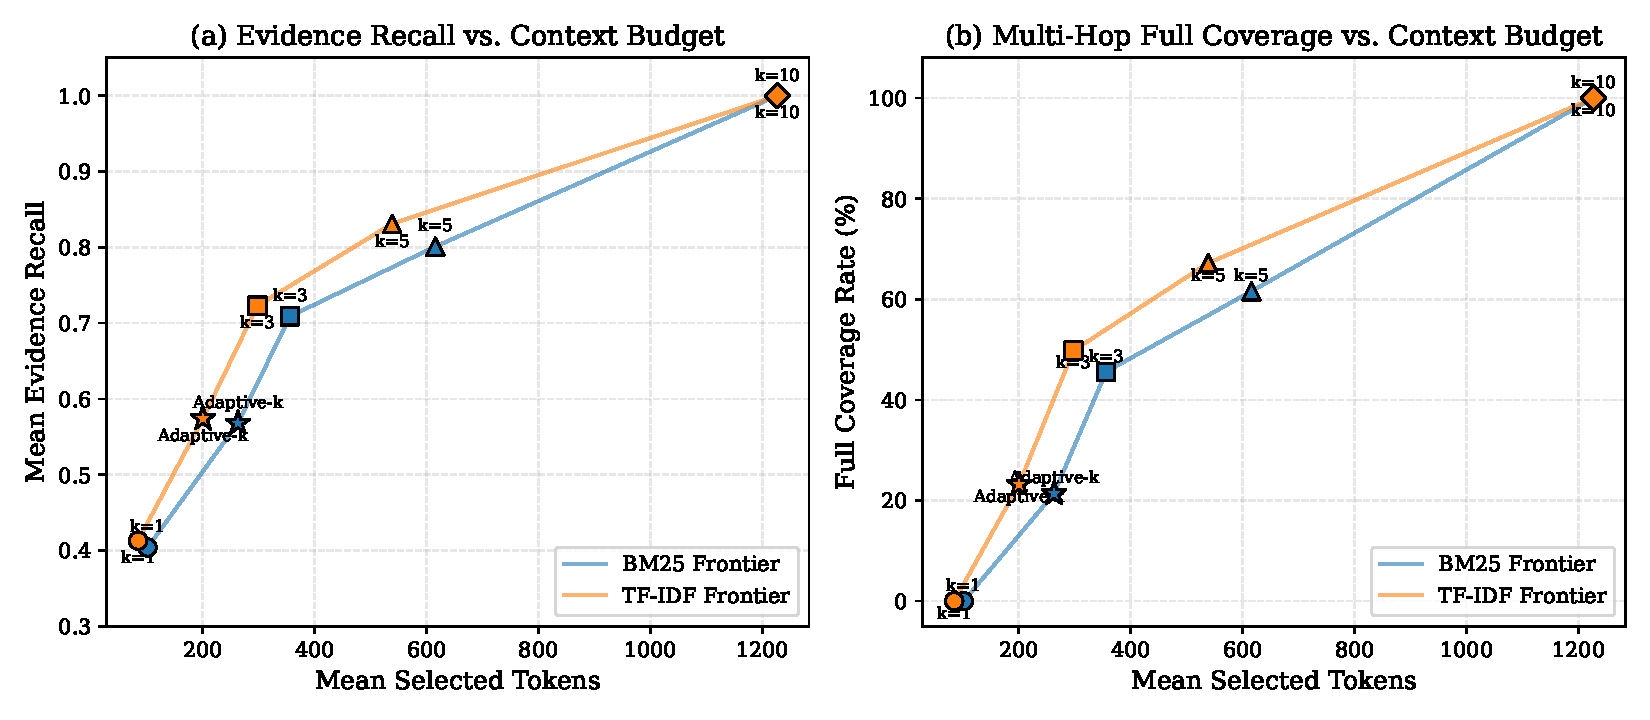
\includegraphics[width=\columnwidth]{figures/figure1_coverage_vs_tokens.pdf}
\caption{Trade-off frontiers between context token consumption and (a) Evidence Recall, and (b) Multi-Hop Full-Coverage Rate for BM25 and TF-IDF.}
\label{fig:pareto}
\end{figure}

\subsection{Evaluation of Pre-Frozen Decision Rules}
\begin{itemize}
    \item \textbf{Decision Rule 1 (Token Efficiency)}: \textit{Score-Gap Adaptive-$k$ Proxy is supported as superior if its 95\% CI for Coverage per 1,000 tokens strictly exceeds all fixed-$k$ configurations.}
    
    \textbf{Verdict: Contradicted / Qualified Negative Result}. While Score-Gap Adaptive-$k$ Proxy dominates fixed $k=3, 5, 10$, fixed $k=1$ achieves a higher coverage-per-token ratio (5.714 for BM25, 6.388 for TF-IDF) due to extreme token brevity ($\sim 85$--$100$ tokens). However, fixed $k=1$ achieves exactly 0.0\% full coverage on multi-hop questions. Thus, while Score-Gap Adaptive-$k$ Proxy forms the most efficient operating point among non-zero full-coverage methods, the strict pre-frozen decision rule is contradicted by the pathological $k=1$ baseline.
    \item \textbf{Decision Rule 2 (Multi-Hop Full Coverage)}: \textit{Score-Gap Adaptive-$k$ Proxy matches fixed $k=5$ full coverage within $\pm 5\%$ while using strictly fewer tokens.}
    
    \textbf{Verdict: Not Supported}. Score-Gap Adaptive-$k$ Proxy achieves only 21.4\% full coverage on BM25 (vs. 61.6\% for fixed $k=5$) and 23.2\% on TF-IDF (vs. 67.2\% for fixed $k=5$).
\end{itemize}

\begin{figure}[t]
\centering
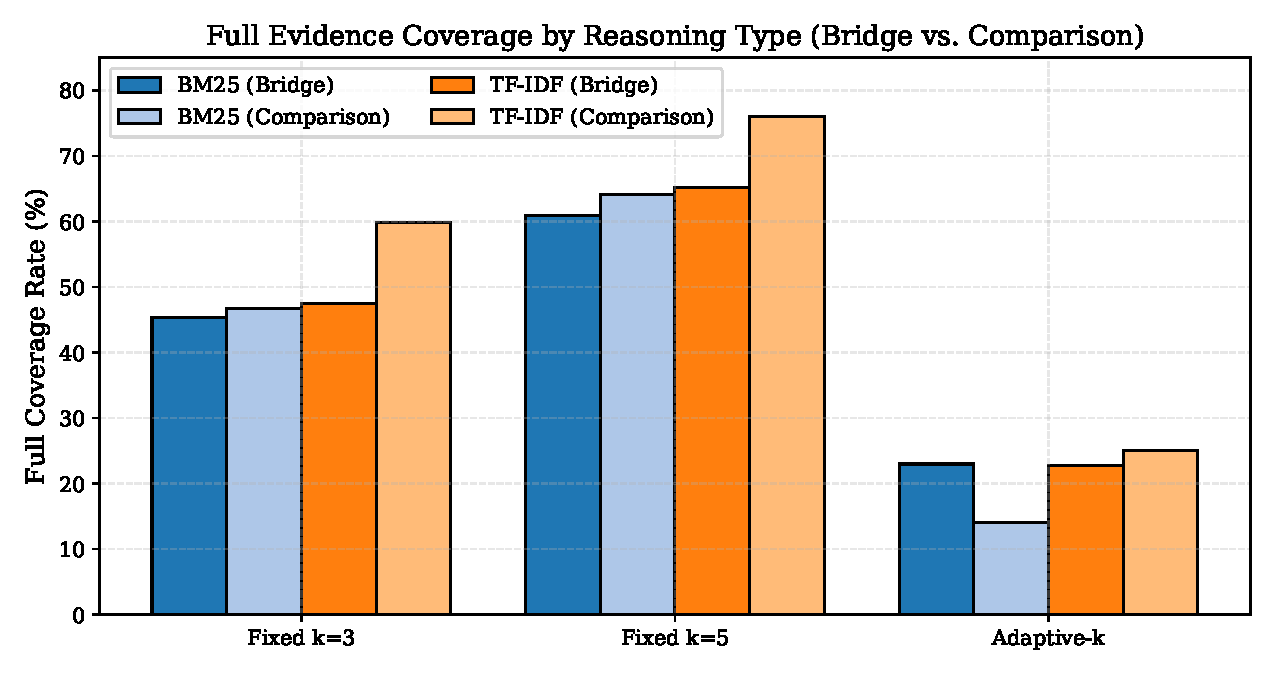
\includegraphics[width=0.9\columnwidth]{figures/figure2_question_types.pdf}
\caption{Full evidence coverage stratified by reasoning type: Bridge vs. Comparison.}
\label{fig:types}
\end{figure}

\subsection{Question Type Breakdown (Figure~\ref{fig:types})}
As illustrated in Figure~\ref{fig:types}, the reported BM25 results show higher full coverage on \textit{Comparison} questions than on \textit{Bridge} questions. For BM25 fixed $k=5$, full coverage on comparison questions reaches 72.8\% compared to 59.1\% on bridge questions. For BM25 Score-Gap Adaptive-$k$ Proxy, full coverage on comparison queries is 29.3\% versus 19.6\% on bridge queries.

\section{Discussion \& Failure Analysis}

\begin{figure}[t]
\centering
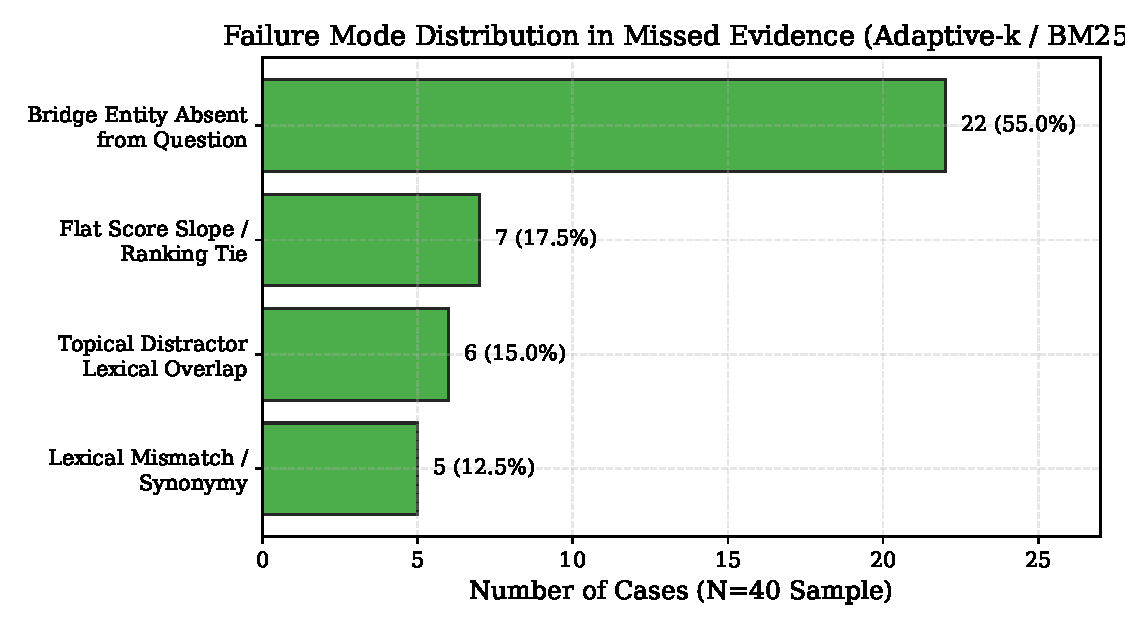
\includegraphics[width=0.88\columnwidth]{figures/figure3_failure_distribution.pdf}
\caption{Failure mode distribution across 40 sampled missed-evidence cases under Score-Gap Adaptive-$k$ Proxy BM25 (Seed 42).}
\label{fig:failures}
\end{figure}

To understand why Score-Gap Adaptive-$k$ Proxy underperforms fixed $k=5$ on multi-hop full coverage, we examined a seeded random sample of 40 missed-evidence cases under BM25 Score-Gap Adaptive-$k$ Proxy (seed 42). Figure~\ref{fig:failures} illustrates the resulting distribution across our pre-frozen categories:
\begin{enumerate}
    \item \textbf{Bridge Entity Absent from Query (55.0\%, $N=22$)}: The predominant failure mode occurs in bridge questions where the query directly mentions only entity $A$. Entity $A$'s paragraph introduces a bridge entity $B$, which is required to answer the question, but entity $B$ never appears in the original query. Consequently, paragraph $A$ scores extremely high while paragraph $B$ receives a low score, causing a sharp score gap immediately after $k=1$ or $k=2$. Score-Gap Adaptive-$k$ Proxy halts before paragraph $B$ can be reached.
    \item \textbf{Flat Score Slope / Ranking Tie (17.5\%, $N=7$)}: When several distractor paragraphs share uniform lexical overlap, the discrete differences $\Delta s_i$ remain near zero, causing premature or fallback cutoffs.
    \item \textbf{Distractor Lexical Overlap (15.0\%, $N=6$)}: Distractors containing superficial repetitions of query keywords outscore the second gold paragraph.
    \item \textbf{Lexical Mismatch / Synonymy (12.5\%, $N=5$)}: The question uses terms not literally present in the Wikipedia lead paragraph.
\end{enumerate}

One possible interpretation of these findings is that single-pass score-gap thresholding can prematurely exclude relevant paragraphs when their similarity to the original query is substantially lower than that of the first-ranked evidence paragraph. This pattern is particularly relevant to bridge questions, where the second-hop entity may not appear explicitly in the original query. This interpretation is consistent with the observed failure categories but does not establish a general property of all multi-hop retrieval systems.

\section{Limitations}
\begin{enumerate}
    \item \textbf{Retrieval-Only Scope}: This study evaluates evidence selection accuracy and token consumption; it does not directly evaluate downstream LLM reader generations or hallucination rates.
    \item \textbf{Benchmark Constraints}: Evaluation was conducted on the distractor setting of HotpotQA ($M=10$ candidates). Performance in full-corpus open-domain retrieval with thousands of candidates remains [TO VERIFY].
    \item \textbf{Sparse Retrievers}: We investigated BM25 and TF-IDF. Dense embeddings with continuous cosine geometries may produce different score distributions.
\end{enumerate}

\section{Conclusion}
This study evaluated fixed-$k$ versus single-pass Score-Gap Adaptive-$k$ Proxy context selection for multi-hop question answering. Our empirical results demonstrate that Score-Gap Adaptive-$k$ Proxy achieves remarkable distractor suppression and token savings (slashing tokens by 78.5\% compared to full context while elevating precision to 74--77\%). However, on multi-hop questions, single-pass score gaps systematically fail to capture latent second-hop evidence paragraphs (achieving only 21.4\% full coverage vs 61.6\% for fixed $k=5$). The question-type analysis shows higher Score-Gap Adaptive-$k$ Proxy full coverage on comparison questions than on bridge questions under BM25 (29.3\% versus 19.6\%). These results indicate that single-pass score-gap selection has limitations in retrieving multi-evidence questions, particularly when second-hop evidence has limited lexical overlap with the original query. Iterative retrieval and query reformulation remain potential directions for future investigation.

\section*{AI-Assistance Disclosure}
In accordance with course directives and research integrity policies, AI assistance (Claude/Gemini via Antigravity) was utilized for code generation, environment diagnostics, and drafting assistance. All experimental executions, data parsing, metric calculations, and failure analyses were executed via local deterministic code in this repository. No synthetic results, p-values, or bibliographic records were generated by AI.

\bibliographystyle{IEEEtran}
\bibliography{references}

\end{document}
